%%%%%%%%%%%%%%%%% SCALING (LA) %%%%%%%%%%%%%%%%%%%%
\begin{figure}[htp]

\begin{subfigure}{\textwidth}
\begin{subfigure}{0.45\textwidth}
\centering
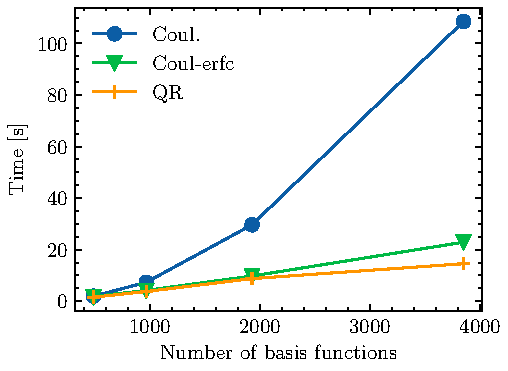
\includegraphics[width=\textwidth]{Pics/hfJ_alkan}
%\label{fig:GS_DFJSCALE_LA}
\end{subfigure}
\hfill
\begin{subtable}{0.45\textwidth}
\centering
\begin{tabular}{rrrr}
\hline
N$_{AO}$ & DFCM & DFCAM & QRDF \\ \hline
490 & --- & --- & --- \\ 
970 & 1.93 & 1.23 & 1.29 \\ 
1930 & 2.03 & 1.23 & 1.23 \\ 
3850 & 1.88 & 1.23 & 0.73 \\ \hline
\end{tabular}
\end{subtable}
\caption{}
%Scaling behavior for the construction of the coulomb matrix using different metrics (LA)}
\label{fig:GS_DFJSCALE_LA}
\end{subfigure}

\vspace{1.5\baselineskip}

\begin{subfigure}{\textwidth}
\begin{subfigure}{0.45\textwidth}
\centering
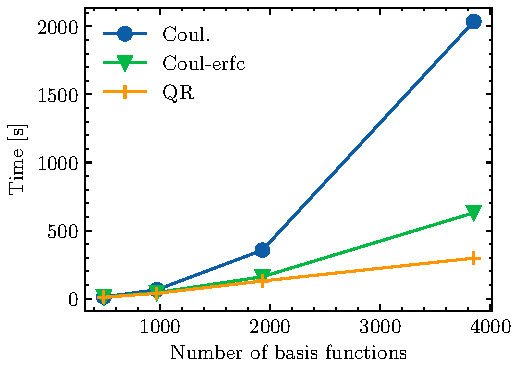
\includegraphics[width=\textwidth]{Pics/hfK1_alkan}
\end{subfigure}
\hfill
\begin{subtable}{0.45\textwidth}
\centering
\begin{tabular}{rrrr}
\hline
N$_{AO}$ & DFCM & DFCAM & QRDF \\ \hline
490 & --- & --- & --- \\ 
970 & 2.43 & 1.97 & 1.96 \\ 
1930 & 2.49 & 1.89 & 1.78 \\ 
3850 & 2.53 & 1.98 & 1.21 \\ \hline
\end{tabular}
\end{subtable}
\caption{}
%Scaling behavior for the construction of the exchange matrix (step1) using different metrics (LA)}
\label{fig:GS_DFK1SCALE_LA}
\end{subfigure}

\vspace{1.5\baselineskip}

\begin{subfigure}{\textwidth}
\begin{subfigure}{0.45\textwidth}
\centering
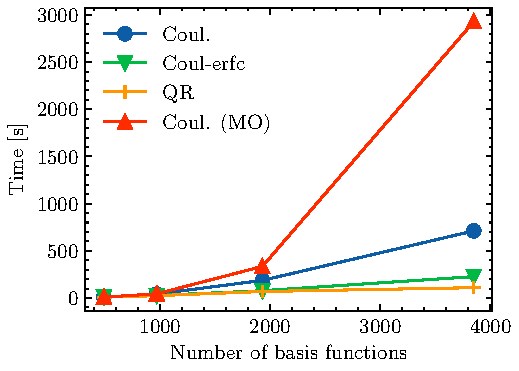
\includegraphics[width=\textwidth]{Pics/hfK2_alkan}
\end{subfigure}
\hfill
\begin{subtable}{0.45\textwidth}
\centering
\resizebox{\textwidth}{!}{
\begin{tabular}{rrrrr}
\hline
N$_{AO}$ & DFCM & DFCAM & QRDF & DFMO \\ \hline
490 & --- & --- & --- & --- \\ 
970 & 1.58 & 1.58 & 1.60 & 2.34 \\ 
1930 & 1.57 & 1.57 & 1.50 & 2.96 \\ 
3850 & 1.56 & 1.56 & 0.67 & 3.14 \\ \hline
\end{tabular}
}
\end{subtable}
\caption{}
%Scaling behavior for the construction of the exchange matrix (step 2) using different metrics (LA)}
\label{fig:GS_DFK2SCALE_LA}
\end{subfigure}
\caption[Scaling behavior of the J and K kernels for LA.]{(a) Scaling behavior for the construction of the coulomb matrix using different metrics (LA). (b) Scaling behavior for the construction of the exchange matrix (step1) using different metrics (LA). (c) Scaling behavior for the construction of the exchange matrix (step 2) using different metrics (LA)}
\end{figure}

%%%%%%%%%%%%%%%%% SCALING (FW) %%%%%%%%%%%%%%%%%%%%%%%

\begin{figure}[htp]

\begin{subtable}{\textwidth}
\resizebox{\textwidth}{!}{
\begin{tabular}{r|rrr|rrr|rrrr}
\hline
 & \multicolumn{3}{c}{J} & \multicolumn{3}{c}{K (STEP 1)} &   \multicolumn{4}{c}{K (STEP 2)} \\ \hline
N$_{AO}$ & DFCM & DFCAM & QRDF & DFCM & DFCAM & QRDF & DFCM & DFCAM & QRDF & DFMO \\ \hline
417 & --- & --- & --- & --- & --- & --- & --- & --- & --- & --- \\ 
777 & 2.18 & 2.20 & 1.88 & 2.77 & 2.77 & 2.51 & 2.55 & 2.55 & 2.33 & 2.33 \\ 
1569 & 2.32 & 1.71 & 1.28 & 2.77 & 2.18 & 1.85 & 2.82 & 2.13 & 1.67 & 2.86 \\ 
3513 & 2.08 & --- & 1.94 & 2.79 & --- & 2.74 & 2.59 & --- & 2.65 & 3.13 \\ \hline
\end{tabular}
}
\caption{}
\label{tab:GS_DFJKSCALE_FW}
\end{subtable}

\vspace{1.5\baselineskip}

\begin{subfigure}{\textwidth}
\centering
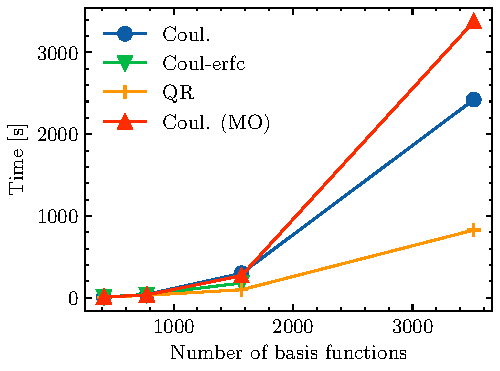
\includegraphics[scale=1.0]{Pics/hfK2_fw}
\caption{}
\label{fig:GS_DFK2SCALE_FW}
\end{subfigure}

\caption[Scaling behavior of the J and K kernels for FW]{(a) Scaling coefficients for the J kernel and the two steps of the K kernel (FW). (b) Scaling for the construction of the exchange matrix (step 2) for hydrated formamide. Although local density approximations do not lower the scaling, a reduction of the prefactor can be observed.}

\end{figure}

%%%%%%%%%%%%%%%%% MEMORY (LA/FW) %%%%%%%%%%%%%%%%%%%%%%%%

%
\begin{figure}[htp]

\begin{subfigure}{\textwidth}
\begin{subfigure}{0.45\textwidth}
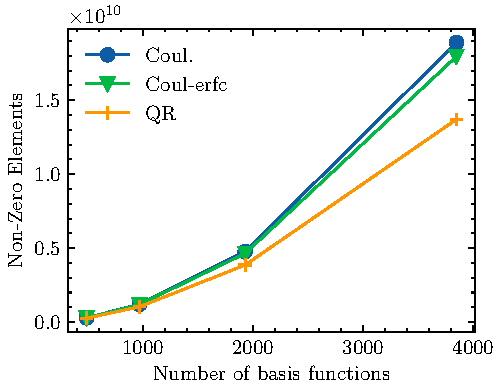
\includegraphics[width=\textwidth]{Pics/cfit_nze_alkan}
\end{subfigure}
\hfill
\begin{subtable}{0.45\textwidth}
\begin{tabular}{rrrr}
\hline
N$_{AO}$ & DFCM & DFCAM & QRDF \\ \hline
490 & --- & --- & --- \\ 
970 & 2.07 & 2.06 & 2.01 \\ 
1930 & 2.01 & 1.98 & 1.92 \\ 
3850 & 1.99 & 1.96 & 1.84 \\ \hline
\end{tabular}
\end{subtable}
\caption{}
\label{fig:GS_MBNZE_LA}
\end{subfigure}

\vspace{1.5\baselineskip}

\begin{subfigure}{\textwidth}
\begin{subfigure}{0.45\textwidth}
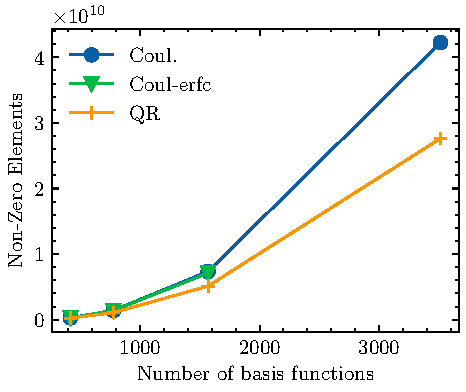
\includegraphics[width=\textwidth]{Pics/cfit_nze_fw}
\end{subfigure}
\hfill
\begin{subtable}{0.45\textwidth}
\begin{tabular}{rrrr}
\hline
N$_{AO}$ & DFCM & DFCAM & QRDF \\ \hline
417 & --- & --- & --- \\ 
777 & 2.27 & 2.26 & 2.20 \\ 
1569 & 1.96 & 1.94 & 1.88 \\ 
3513 & 1.71 & 1.68 & 1.57 \\ \hline
\end{tabular}
\end{subtable}
\caption{}
\label{fig:GS_MBNZE_FW}
\end{subfigure}
%

\caption[Scaling behavior of the tensor $M_{XY}B_{Y\mu\nu}$]{(a) Scaling behavior of the tensor $M_{XY}B_{Y\mu\nu}$ (LCA). (b) Scaling behavior of the tensor $M_{XY}B_{Y\mu\nu}$ (FW).}

\end{figure}